% WORKAROUND (an update of the geometry package broke beamer...)
\makeatletter\let\ifGm@compatii\relax\makeatother
% end of WORKAROUND


\documentclass{beamer}
% \usetheme[uttitlepage=false]{ut}
\usetheme[euler=false,titlepage=C]{ut}
\usetheme{ut}

\usepackage{tikz-cd}
\usepackage[most]{tcolorbox}

\usepackage[backend=bibtex, style=authoryear, doi=false,isbn=false,url=false]{biblatex}

\usepackage{bm}
\usepackage{color}
\definecolor{theme}{RGB}{0,73,114}

\usepackage{graphicx}
\usepackage{diffcoeff}
\usepackage[most]{tcolorbox}
\usepackage{mathtools}

\usepackage[beamer]{hf-tikz}
\usetikzlibrary{calc}

% Math macros
\DeclareMathOperator*{\grad}{grad}
\DeclareMathOperator*{\Grad}{Grad}
\DeclareMathOperator*{\Div}{Div}
\renewcommand{\div}{\operatorname{div}}
\DeclareMathOperator*{\Hess}{Hess}
\DeclareMathOperator*{\curl}{curl}
\DeclareMathOperator{\Tr}{Tr}
\DeclareMathOperator{\Dom}{Dom}
\DeclareMathOperator*{\esssup}{ess\,sup}

\newcommand{\bbR}{\mathbb{R}}
\newcommand{\bbF}{\mathbb{F}}
\newcommand{\bbA}{\mathbb{A}}
\newcommand{\bbB}{\mathbb{B}}
\newcommand{\bbS}{\mathbb{S}}

\newcommand*{\norm}[1]{\ensuremath{\left\|#1\right\|}}
\newcommand{\where}{\qquad \text{where} \qquad}
\newcommand{\inner}[3][]{\ensuremath{\left\langle #2, \, #3 \right\rangle_{#1}}}
\newcommand{\bilprod}[2]{\left\langle \left\langle \, #1, #2 \, \right\rangle \right\rangle}
\newcommand{\pder}[2]{\ensuremath{\partial_{#2} #1}}
\newcommand{\dder}[2]{\ensuremath{\delta_{#2} #1}}
\newcommand{\secref}[1]{\S\ref{#1}}
\newcommand{\energy}[1]{\frac{1}{2} \int_{\Omega} \left\{ #1 \right\} \d\Omega}
\newcommand{\crmat}[1]{\ensuremath{\left[#1\right]_\times}}
\newcommand{\fenics}{\textsc{FEniCS}\xspace}
\newcommand{\firedrake}{\textsc{Firedrake}\xspace}

\DeclareMathOperator*{\argmax}{arg\,max}
\DeclareMathOperator*{\argmin}{arg\,min}

\newtheorem{proposition}{Proposition}
\newtheorem{remark}{Remark}
\newtheorem{hypothesis}{Hypothesis}
\newtheorem{assumption}{Assumption}
\newtheorem{conjecture}{Conjecture}


\def\onedot{$\mathsurround0pt\ldotp$}
\def\cddot{% two dots stacked vertically
	\mathbin{\vcenter{\baselineskip.67ex
			\hbox{\onedot}\hbox{\onedot}}%
}}

\renewcommand\bibfont{\scriptsize}


\makeatletter \renewcommand\d[1]{\ensuremath{%
		\;\mathrm{d}#1\@ifnextchar\d{\!}{}}}
\makeatother


\graphicspath{{./images/}}

\bibliography{./biblio_LHMNC}


%% At begin of each section: show current section and all subsections in the section if any
%% At begin of each subsection except first: show only the current section/subsection
\newif\iftocsub
\tocsubtrue
\AtBeginSection[] {
	\begin{frame}[noframenumbering]{Outline}
		\tableofcontents[sectionstyle=show/shaded, subsectionstyle=show/show/hide]
	\end{frame}
	\tocsubfalse
}
\AtBeginSubsection[] {
	\iftocsub
	\begin{frame}[noframenumbering]{Outline}
		\tableofcontents[currentsubsection, sectionstyle=show/shaded, subsectionstyle=show/shaded/hide]
	\end{frame}
	\fi
	\tocsubtrue
}


\title{Mixed finite elements for port-Hamiltonian models of von Kármán beams\\
	\small{7th IFAC Conference on Lagrangian and Hamiltonian method for non linear control}}
%  
\institute[UT]{\inst{1}University of Twente, Enschede (NL) \and \inst{2}ISAE-SUPAERO, Toulouse (FR)}

% \subtitle[Short subtitle]{I am not using any subtitles}
\author[A.~Brugnoli]{Andrea Brugnoli\inst{1} \and Ramy Rashad\inst{1} \and Federico Califano\inst{1} \and Stefano Stramigioli\inst{1} \and Denis Matignon\inst{2} } 

\date{\flushright 11-13 October, 2021}
\footlinetext{[A.~Brugnoli]}
% \titlegraphic{\includegraphics[height=1cm]{titlegraphic}}

\utbeamerset{tpboxax=5, tpboxay=20, tpboxawd=100, tpboxbht=30, tpboxbx=5, tpboxby=35, tpboxbwd=120, tpboxbht=30,}

\begin{document}

\maketitle

\begin{frame}{Overview}
	\tableofcontents
\end{frame}

\section{Von-Karman theory of thin beams/plates}

\begin{frame}{Linear vs Von-K\`arm\`an plate theory}

	\begin{columns}
	\begin{column}{.5\textwidth}
			\includegraphics[width=1\columnwidth]{buckling.jpg}
	\end{column}
	\begin{column}{.5\textwidth}

		Non linearity allows to describe bifurcations, i.e. buckling.
	\end{column}
	\end{columns}
	
\end{frame}

\begin{frame}{The von-K\`arm\`an assumption}
		
\begin{block}{Basic geometric assumption}
	Out of plane deflection comparable compared to the thickness: $w/h = \mathcal{O}(1)$. \\
\end{block}

\begin{columns}
	\begin{column}{.55\textwidth}
		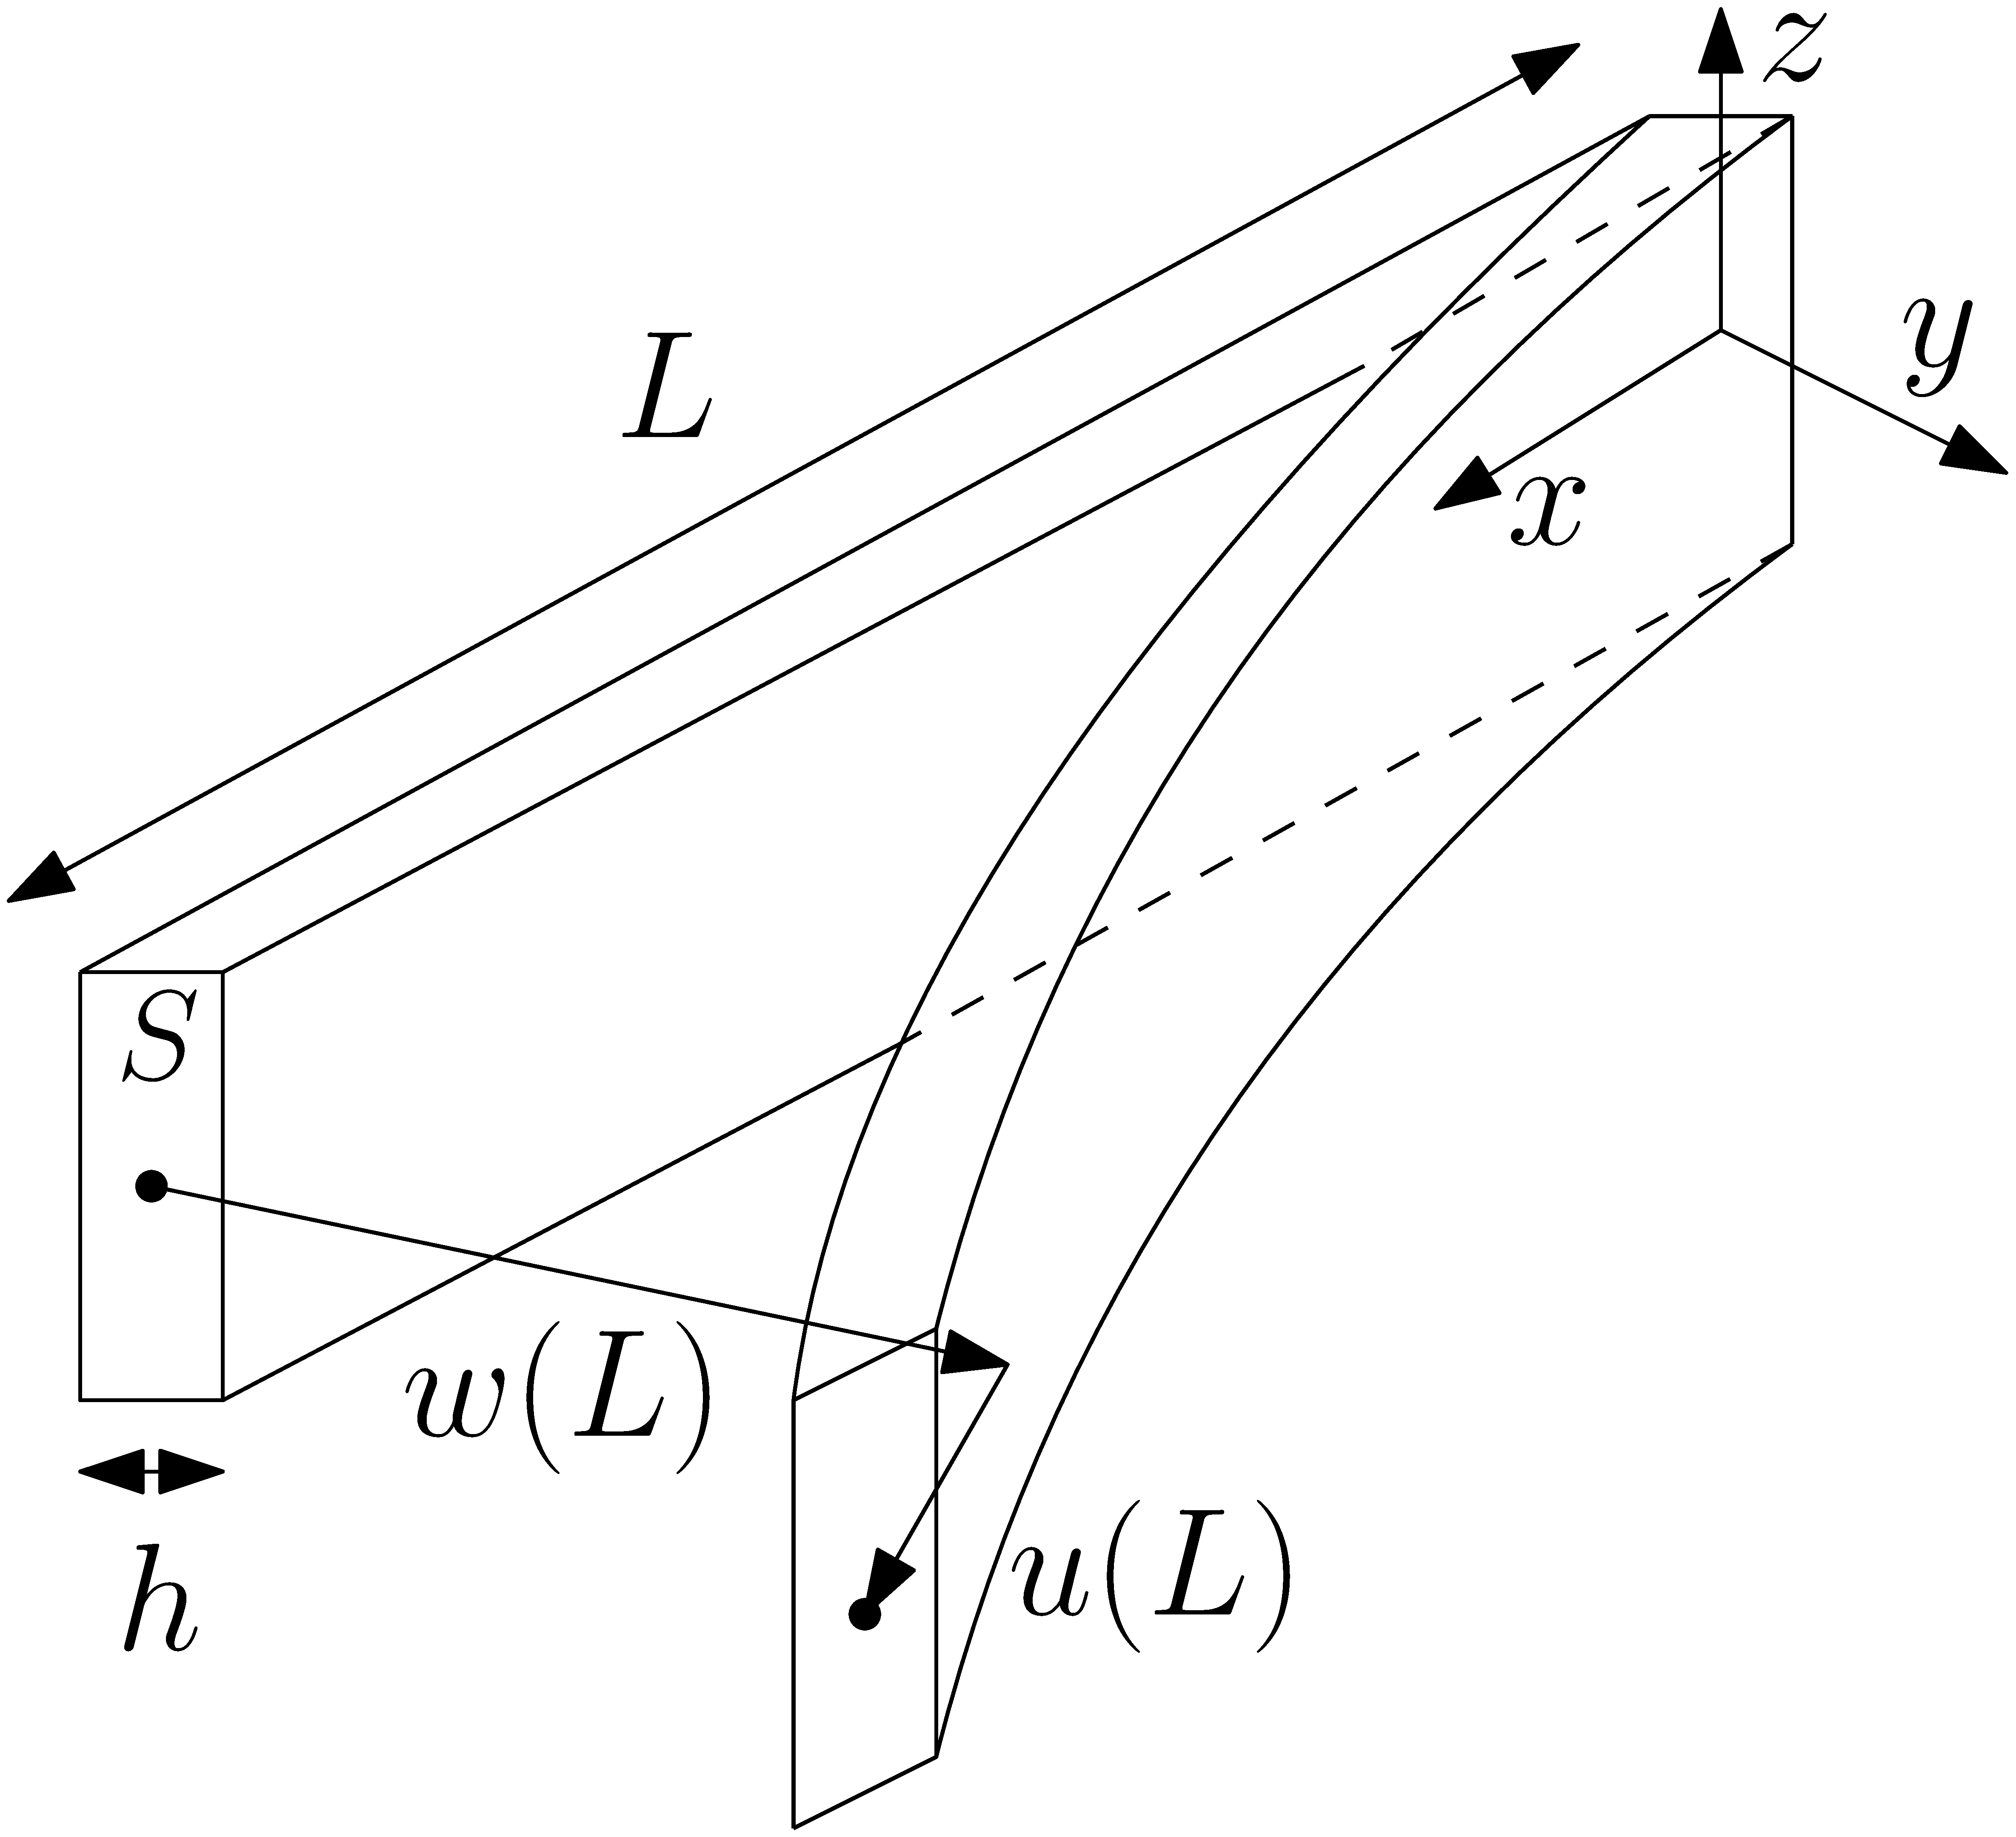
\includegraphics[width=1\columnwidth]{beam_deflected.eps}
	\end{column}
	\begin{column}{.45\textwidth}
		Aspect ratio: $\delta= h/L$.
		
		The following terms are kept in the expansion:
		\begin{equation*}
		\begin{aligned}
			w/L &= \mathcal{O}(\delta), \\
			u/L &= \mathcal{O}(\delta^2), \\
		\end{aligned}
		\end{equation*}
	\end{column}
\end{columns}

\end{frame}

\begin{frame}{Stresses and Strains}
	
Decomposition strain field 
\begin{equation*}
	\varepsilon_{xx} = \overbrace{\tikzmarkin<1>[below right offset={0.05,-0.4},above left offset={-0.05,0.7}]{lm}\diffp{u}{x}\tikzmarkend{lm} +  \tikzmarkin<1>[below right offset={0,-0.4},above left offset={-0.05,0.7}]{nlm}\frac{1}{2} \left(\diffp{w}{x} \right)^2\tikzmarkend{nlm}}^{\varepsilon_{xx}^m} - \overbrace{\tikzmarkin<1>[below right offset={0.05,-0.4},above left offset={-0.05,0.7}]{lb}z\diffp[2]{w}{x}\tikzmarkend{lb}}^{\kappa_{xx}}
\end{equation*}

\begin{tikzpicture}[remember picture,overlay]
	% adjust the shift from "col" to move the position of the annotation
	\coordinate (lm-a) at ($(lm)+(-2,-2)$);
	\coordinate (lm-b) at ($(lm)+(0.4,-1.1)$);
	\node[align=left] (lmstring) at (lm-a) {\small{Linear membrane def.}};
	\draw[->, red](lmstring) -| node {} (lm-b);
	
	\coordinate (nlm-a) at ($(nlm)+(-3.3,-3)$);
	\coordinate (nlm-b) at ($(nlm)+(0.8,-1.1)$);
	\node[align=left] (nlmstring) at (nlm-a) {\small{Non-linear membrane def.}};
	\draw[->, red](nlmstring) -| node {} (nlm-b);
	
	\coordinate (lb-a) at ($(lb)+(+2,-3)$);
	\coordinate (lb-b) at ($(lb)+(0.3,-1.1)$);
	\node[align=right] (lbstring) at (lb-a) {\small{Linear bending def.}};
	\draw[->, red](lbstring) -| node {} (lb-b);
	
\end{tikzpicture}

\end{frame}

\begin{frame}{Membrane-bending problem for thin beams}
	
For small deformations the membrane and bending behavior are uncoupled:

\begin{equation*}
		\diffp{}{t}
		\begin{pmatrix}
			\alpha_u \\
			\alpha_\varepsilon \\
			\alpha_w \\
			\alpha_\kappa			
		\end{pmatrix} = 
	\begin{bmatrix}
	0 & \partial_x & 0 & 0 \\
	\partial_x & 0 & 0 & 0 \\
	0 & 0 & 0 & -\partial_{xx} \\
	0 & 0 & \partial_{xx} & 0 \\
 	\end{bmatrix}
 \begin{pmatrix}
 	e_u \\
 	e_\varepsilon \\
 	e_w \\
 	e_\kappa			
 \end{pmatrix}
\end{equation*}
 If the material is isotropic 

\end{frame}


\begin{frame}[allowframebreaks]{References}
	\printbibliography
\end{frame}






\end{document}

